% p1 main LaTeX source — Springer LNCS/CCIS one-column.
% Reverse-engineered from p1/latex/isds2026_paper.pdf via pdftotext.
% Ligatures (fi, ffi, fl) restored; section structure preserved.

\documentclass[runningheads]{llncs}

\usepackage[T1]{fontenc}
\usepackage[utf8]{inputenc}
\usepackage{graphicx}
\usepackage{booktabs}
\usepackage{amsmath}
\usepackage{amssymb}
\usepackage{array}
\usepackage{tikz}
\usetikzlibrary{positioning,arrows.meta,shapes.geometric,fit,backgrounds,calc}
\usepackage{pgfplots}
\pgfplotsset{compat=1.18}
\usepackage{hyperref}

% Draft watermark — remove before camera-ready.
\usepackage{draftwatermark}
\SetWatermarkText{DRAFT}
\SetWatermarkScale{5}
\SetWatermarkLightness{0.88}
\SetWatermarkColor[rgb]{0.80,0.15,0.15}

% Okabe-Ito Color Universal Design (CUD) palette — colourblind-safe.
\definecolor{CUDOrange}{HTML}{E69F00}
\definecolor{CUDSkyBlue}{HTML}{56B4E9}
\definecolor{CUDBluishGreen}{HTML}{009E73}
\definecolor{CUDBlue}{HTML}{0072B2}
\definecolor{CUDVermilion}{HTML}{D55E00}
\definecolor{CUDYellow}{HTML}{F0E442}

\begin{document}

\title{The Impact of Prompt Quality on Generative AI Response Quality: A Controlled Experiment with IT Students}

\titlerunning{Prompt Quality Impact on GenAI Response}

\author{Ngoc-My-Quyen Nguyen\inst{1} \and Khuong Ho-Van\inst{2} \and Thanh-Phong Lam\inst{3}}

\authorrunning{N.M.Q. Nguyen et al.}

\institute{FPT University, Ho Chi Minh City, Vietnam \\
\email{quyennnm25ms23295@fpt.edu.vn}
\and Ho Chi Minh City University of Technology (HCMUT), Vietnam \\
\email{hvkhuong@hcmut.edu.vn}
\and Banking University of Ho Chi Minh City, Vietnam \\
\email{020201240024@st.buh.edu.vn}}

\maketitle

\InputIfFileExists{pilot-macros}{}{%
  \newcommand{\PilotN}{TBD}%
  \newcommand{\PilotSessions}{TBD}%
  \newcommand{\PilotFriedmanChi}{TBD}%
  \newcommand{\PilotFriedmanDF}{TBD}%
  \newcommand{\PilotFriedmanP}{TBD}%
  \newcommand{\PilotKendallW}{TBD}%
  \newcommand{\PilotAlgoBasic}{TBD}%
  \newcommand{\PilotAlgoInt}{TBD}%
  \newcommand{\PilotAlgoAdv}{TBD}%
  \newcommand{\PilotCxBasic}{TBD}%
  \newcommand{\PilotCxInt}{TBD}%
  \newcommand{\PilotCxAdv}{TBD}%
  \newcommand{\PilotPsBasic}{TBD}%
  \newcommand{\PilotPsInt}{TBD}%
  \newcommand{\PilotPsAdv}{TBD}%
}

\begin{abstract}
The rapid adoption of generative artificial intelligence (GenAI) tools such as ChatGPT and Claude among university students has raised a critical pedagogical question: does the quality of user-written prompts significantly influence the quality of AI-generated responses? Despite growing evidence that prompt engineering matters, most existing studies examine only a single AI platform, rely on uncontrolled observations, and are situated exclusively in Western educational contexts. This paper presents the design of a controlled within-subjects experiment to quantify the impact of prompt quality on GenAI response efficacy across two competing platforms---OpenAI's GPT-4o-mini and Zhipu AI's GLM-5.1---in the context of IT students performing academic learning tasks at a Vietnamese university. We operationalize prompt quality into three levels (basic, intermediate, advanced) guided by the CLEAR framework and measure response quality using a proposed five-dimensional AI Output Quality Rubric (AIOQ-R) covering accuracy, completeness, relevance, clarity, and learning value. The experimental design employs a Two-Way Repeated-Measures ANOVA with Latin Square counterbalancing ($N = 30$--$40$), complemented by semi-structured interviews analyzed through thematic analysis. We hypothesize that higher prompt quality produces significantly better AI responses (partial $\eta^2 \geq 0.06$) and that platform-specific differences emerge across task types. To the authors' knowledge, this study contributes one of the earliest cross-platform controlled experimental designs in a Southeast Asian educational setting, a validated assessment rubric, and practical prompt-writing guidelines for IT students.

\keywords{prompt engineering \and generative AI \and response quality \and AIOQ-R rubric \and higher education \and CLEAR framework}
\end{abstract}

\section{Introduction}

The proliferation of generative AI tools---including OpenAI's ChatGPT, Anthropic's Claude, and Google's Gemini---has fundamentally transformed how university students approach learning and research. A global survey by the Digital Education Council~\cite{DEC2024}, encompassing over 3{,}800 students across 16 countries, reported that GenAI adoption in academic contexts has exceeded 86\%, with computer science students leading at approximately 91\%. A UK-based longitudinal survey by HEPI~\cite{HEPI2025} ($n = 1{,}041$) further documented that daily ChatGPT usage among students rose from 53\% in 2023 to 66\% in 2024, with the primary use cases being conceptual explanation (68\%), writing assistance (57\%), and programming support (54\%).

However, a fundamental challenge persists: the quality of AI-generated responses is heavily contingent upon the quality of user-supplied prompts. GenAI does not automatically become an effective learning tool merely through access; its pedagogical utility depends critically on the user's interaction competence. Knoth et al.~\cite{Knoth2024} demonstrated through regression analysis that prompt quality serves as a key mediator in the causal chain: AI literacy $\rightarrow$ prompt quality $\rightarrow$ LLM output quality. Sawalha et al.~\cite{Sawalha2024} analyzed 201 authentic student--ChatGPT conversations and found that 26\% of students simply copied assignment instructions verbatim without contextual elaboration, resulting in shallow responses. Two improved prompting strategies---reformulation and multi-question---yielded significantly higher accuracy with Cohen's $d$ values of $-0.94$ and $-0.69$, respectively.

Converging evidence from recent studies reinforces these findings. Kumar et al.~\cite{Kumar2025} reported that engineering students trained in structured prompt techniques achieved up to 33\% higher scores on data analysis and programming tasks compared to unguided peers. Woo et al.~\cite{Woo2025} confirmed that systematic prompt engineering interventions significantly improved both self-efficacy and actual prompt quality among higher education students. These results collectively indicate that prompt literacy training constitutes a measurable educational intervention.

Despite these advances, three critical research gaps remain. \emph{First}, the vast majority of existing studies examine only a single AI platform (predominantly ChatGPT), precluding cross-platform comparisons---even though students routinely use multiple tools and need evidence-based guidance on platform selection. \emph{Second}, the entire body of literature is concentrated in Western educational contexts; no controlled study has been conducted in Southeast Asia, despite comparable GenAI adoption rates among Vietnamese engineering students~\cite{Bui2025}. \emph{Third}, there is a conspicuous absence of validated, multi-dimensional assessment instruments---most studies employ ad hoc scales measuring only accuracy, neglecting educationally significant dimensions such as learning value.

To address these gaps, the present study proposes a controlled within-subjects experiment examining the impact of prompt quality on AI response quality across two platforms (GPT-4o-mini and GLM-5.1) in the context of IT learning tasks at a Vietnamese university. The study is guided by three research questions:

\begin{itemize}
  \item \textbf{RQ1:} To what extent do three levels of prompt quality (basic, intermediate, advanced) affect AI response quality, as measured by the five dimensions of the AIOQ-R rubric?
  \item \textbf{RQ2:} Are there statistically significant differences in response quality between GPT-4o-mini and GLM-5.1 under identical prompt conditions?
  \item \textbf{RQ3:} Is there a significant interaction effect between prompt quality level and AI platform on response quality across different IT task types?
\end{itemize}

Based on the theoretical framework and prior empirical evidence~\cite{Knoth2024,Sawalha2024,Kumar2025}, we propose three hypotheses:

\begin{itemize}
  \item \textbf{H1 (Main effect---Prompt Quality):} Prompt quality level has a statistically significant effect on composite AIOQ-R scores, with the expected ordering: advanced $>$ intermediate $>$ basic (anticipated partial $\eta^2 \geq 0.06$).
  \item \textbf{H2 (Main effect---Platform):} There is a statistically significant difference in composite AIOQ-R scores between GPT-4o-mini and GLM-5.1 under identical prompt conditions. This hypothesis is exploratory.
  \item \textbf{H3 (Interaction effect):} There is a significant interaction between prompt quality level and AI platform, with GLM-5.1 expected to show greater sensitivity to prompt structural completeness and GPT-4o-mini a flatter ceiling on compact tasks.
\end{itemize}

This paper makes three contributions: (1) to the authors' knowledge, among the earliest controlled cross-platform experimental designs for studying prompt--response dynamics in a Southeast Asian educational setting; (2) a proposed five-dimensional AIOQ-R rubric with a planned validation protocol (CVI $\geq 0.80$, $\kappa \geq 0.70$); and (3) an integrated theoretical framework combining the CLEAR framework, Cognitive Load Theory~\cite{Sweller1988}, and TAM2~\cite{Davis1989,Venkatesh2000} to explain the prompt--response mechanism.

The remainder of this paper is organized as follows. Section~\ref{sec:related} reviews related work. Section~\ref{sec:method} details the proposed methodology. Section~\ref{sec:results} presents expected results, followed by a discussion in Section~\ref{sec:discussion}. Section~\ref{sec:conclusion} concludes the paper.

\section{Related Work}\label{sec:related}

\subsection{Generative AI and LLMs in Education}

Generative AI (GenAI) refers to a class of artificial intelligence systems capable of producing novel content---text, code, images---based on patterns learned from large-scale training data. The underlying technology, large language models (LLMs), employs the Transformer architecture trained on massive text corpora to perform diverse tasks including question answering, text summarization, and code generation~\cite{Brown2020,Bommasani2021}. A defining characteristic of LLMs is their sensitivity to input prompts, which serve as the primary mechanism for directing the model's generation process.

In higher education, GenAI tools have been rapidly integrated into student workflows. Sun et al.~\cite{Sun2024} analyzed screen recordings of 30 CS students interacting with ChatGPT and identified three strategy groups: passive copy-paste users, simple sequential interactors, and multi-turn critical engagers---with the last group achieving the highest learning outcomes. Knoth et al.~\cite{Knoth2024} provided quantitative evidence that students with higher AI literacy write better prompts and receive higher-quality AI responses. However, Kasneci et al.~\cite{Kasneci2023} warned that over-reliance on GenAI may erode critical thinking, independent problem-solving, and active knowledge construction---a counterpoint that optimistic studies frequently overlook.

\subsection{Prompt Engineering and the CLEAR Framework}

Prompt engineering is defined as the systematic design and optimization of input instructions to maximize the quality of AI-generated outputs~\cite{Sahoo2024}. Established techniques include Zero-Shot, Few-Shot, Chain-of-Thought (CoT), Role Prompting, and Iterative Prompting. Zlatkin-Troitschanskaia et al.~\cite{Zlatkin2024} proposed a theoretical framework positioning prompt engineering as a 21st-century skill comprising four components: foundational prompt knowledge, prompt read-write ability, prompt methodology, and online critical thinking. Lee and Palmer~\cite{Lee2025} conducted a systematic review of 42 studies and concluded that this skill remains largely absent from formal university curricula despite increasing demand.

The CLEAR framework, proposed by Lo~\cite{Lo2023}, defines five criteria for high-quality prompts: Concise, Logical, Explicit, Adaptive, and Reflective. With over 200 citations, CLEAR provides a principled basis for operationalizing prompt quality into ordinal levels. In this study, we adopt CLEAR to define three prompt quality tiers: Level~1 (basic, satisfying 0--1 CLEAR criteria), Level~2 (intermediate, 2--3 criteria), and Level~3 (advanced, 4--5 criteria).

\subsection{Prompt Sensitivity and Output Quality}

LLMs exhibit high sensitivity to prompt wording, structure, and formatting. Minor variations in phrasing can produce substantially different outputs~\cite{Zhao2021}, and techniques such as CoT prompting have demonstrated that explicit reasoning instructions markedly improve problem-solving performance~\cite{Wei2022}. Brown et al.~\cite{Brown2020} showed that LLMs leverage in-context learning, where the prompt functions as a task specification that shapes the entire generation trajectory.

Knoth et al.~\cite{Knoth2024} provided the first empirical evidence for a causal chain: AI Literacy $\rightarrow$ Prompt Quality $\rightarrow$ LLM Output Quality, coding prompts along six components (task verb, focus, context, constraints, output specification, reasoning instruction). Sawalha et al.~\cite{Sawalha2024} confirmed that students who copied assignment text verbatim received significantly lower-quality responses compared to those using reformulation ($d = -0.94$) or multi-question strategies ($d = -0.69$). Kumar et al.~\cite{Kumar2025} demonstrated a 33\% performance advantage for students trained in structured prompting. Choi et al.~\cite{Choi2025} analyzed 1{,}259 student prompts across 12 STEM courses and identified eight quality factors, with context and output constraints carrying the highest predictive weight.

\subsection{Evaluation Frameworks for AI-Generated Content}

Several frameworks have been developed to assess AI output quality. Huang et al.~\cite{Huang2025} developed the AIGDER index using Delphi and Analytic Hierarchy Process (AHP) methods, identifying four priority dimensions: authenticity, accuracy, relevance, and depth. Goodman et al.~\cite{Goodman2023} proposed a 6-point accuracy scale and a 3-point completeness scale that have been widely adapted. Liu et al.~\cite{Liu2023} introduced G-Eval, which uses GPT-4 itself as an evaluator across dimensions of relevance, coherence, consistency, and fluency.

However, most existing instruments measure only surface-level accuracy and lack systematic inter-rater reliability testing. Critically, no validated rubric incorporates \emph{learning value}---the degree to which AI responses stimulate higher-order thinking (Bloom's taxonomy)---as an assessment dimension. The AIOQ-R rubric proposed in this study addresses this gap with a five-dimensional evaluation covering accuracy, completeness, relevance, clarity, and learning value, accompanied by anchor examples and a planned validation protocol.

\subsection{Research Gaps}

From the literature review, four gaps emerge:

\begin{itemize}
  \item \textbf{Gap 1:} No study has compared the impact of prompt quality across multiple AI platforms (e.g., ChatGPT vs. Claude) under controlled experimental conditions.
  \item \textbf{Gap 2:} Research is overwhelmingly concentrated in Western contexts; few peer-reviewed controlled studies have been reported in Southeast Asia despite comparable adoption rates~\cite{Bui2025}.
  \item \textbf{Gap 3:} The relationship between prompt quality and \emph{learning value}---beyond surface-level response quality---has not been systematically measured, including the potential negative effects of over-reliance on higher-order thinking.
  \item \textbf{Gap 4:} There is no validated, multi-dimensional rubric with established reliability for assessing AI response quality in the context of IT learning tasks.
\end{itemize}

This study is positioned to address all four gaps simultaneously through a controlled cross-platform experiment with a validated assessment instrument.

\begin{figure}[!t]
\centering
\resizebox{\textwidth}{!}{%
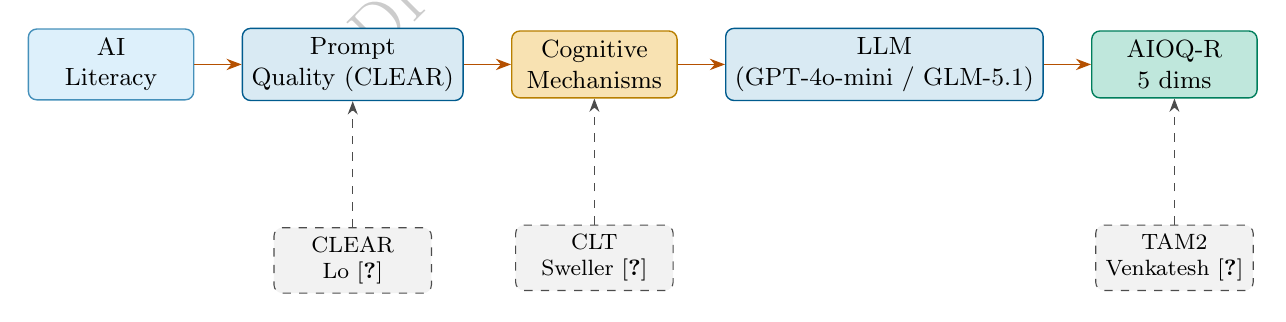
\begin{tikzpicture}[
  node distance=0.6cm and 0.6cm,
  box/.style={rectangle, draw, rounded corners=3pt, minimum width=2.1cm, minimum height=0.85cm, align=center, font=\small, line width=0.5pt},
  boxIn/.style={box, fill=CUDSkyBlue!20, draw=CUDSkyBlue!80!black},
  boxProc/.style={box, fill=CUDBlue!15, draw=CUDBlue!80!black},
  boxEmp/.style={box, fill=CUDOrange!30, draw=CUDOrange!80!black},
  boxOut/.style={box, fill=CUDBluishGreen!25, draw=CUDBluishGreen!80!black},
  theo/.style={rectangle, draw=gray!60!black, dashed, rounded corners=3pt, minimum width=2.0cm, minimum height=0.7cm, align=center, font=\footnotesize, fill=gray!10},
  arr/.style={->, thick, >=Stealth, draw=CUDVermilion!85!black, line width=0.55pt},
  tarr/.style={->, dashed, >=Stealth, draw=gray!60!black}
]
\node[boxIn]                     (lit)  {AI\\Literacy};
\node[boxProc, right=of lit]     (pq)   {Prompt\\Quality (CLEAR)};
\node[boxEmp,  right=of pq]      (mech) {Cognitive\\Mechanisms};
\node[boxProc, right=of mech]    (llm)  {LLM\\(GPT-4o-mini / GLM-5.1)};
\node[boxOut,  right=of llm]     (out)  {AIOQ-R\\5 dims};

\draw[arr] (lit) -- (pq);
\draw[arr] (pq) -- (mech);
\draw[arr] (mech) -- (llm);
\draw[arr] (llm) -- (out);

\node[theo, below=1.6cm of pq]   (clear) {CLEAR\\Lo~\cite{Lo2023}};
\node[theo, below=1.6cm of mech] (clt)   {CLT\\Sweller~\cite{Sweller1988}};
\node[theo, below=1.6cm of out]  (tam)   {TAM2\\Venkatesh~\cite{Venkatesh2000}};

\draw[tarr] (clear) -- (pq);
\draw[tarr] (clt)   -- (mech);
\draw[tarr] (tam)   -- (out);
\end{tikzpicture}%
}
\caption{Integrated theoretical framework. The causal chain (top row, solid) extends Knoth et al.~\cite{Knoth2024} by inserting three cognitive mechanisms---\{Ambiguity Reduction, Task Representation, Reasoning Scaffolding\}---between prompt quality and LLM output. Three supporting theories (bottom, dashed) ground the operationalisation.}
\label{fig:framework}
\end{figure}

\section{Methodology}\label{sec:method}

Figure~\ref{fig:framework} situates the study within an integrated theoretical model: AI literacy predicts prompt quality operationalised by CLEAR, which activates three cognitive mechanisms that shape LLM output along the AIOQ-R dimensions.

\subsection{Research Design}

This study employs a Sequential Explanatory Mixed Methods design~\cite{Creswell2018}. Phase~1 (quantitative) consists of a controlled within-subjects experiment, followed by Phase~2 (qualitative) comprising semi-structured interviews to explain and enrich the quantitative findings. This design is appropriate because: (1) the experiment provides objective measurements of prompt effects; (2) interviews capture student perceptions and experiences that quantitative measures cannot fully reflect; and (3) the sequential approach has been successfully validated in analogous studies~\cite{Woo2025,Kumar2025}.

\subsection{Participants and Sample Size}

Participants are third- and fourth-year IT students at a technology-oriented university in Vietnam, with experience using at least one GenAI tool. The target sample size is $N = 30$--$40$, determined through a priori power analysis using G*Power 3.1 with the following parameters: significance level $\alpha = 0.05$; statistical power $1 - \beta = 0.80$; medium effect size $f = 0.25$ (equivalent to partial $\eta^2 \approx 0.06$, conservatively below $d = 0.69$ reported by Sawalha et al.~\cite{Sawalha2024}). For a Two-Way Repeated-Measures ANOVA design (Prompt Level $\times$ Platform; $3 \times 2 = 6$ conditions), the minimum required sample is $N = 28$ under the standard G*Power assumption of a nonsphericity correction $\epsilon = 1$ and a within-subject correlation among repeated measures $\rho \geq 0.5$. A sensitivity analysis at $\rho = 0.3$ raises the required $N$ to approximately 45; we therefore treat $N = 28$ as a lower bound, target $N = 30$--$40$ to buffer attrition and data exclusion, and pre-specify that if the observed $\rho$ falls below 0.5 we will recruit a second wave before testing H3 (interaction effect).

\subsection{Variables and Instruments}

\textbf{Independent Variable (IV):} Prompt quality, operationalized at three levels based on the CLEAR framework~\cite{Lo2023} and the six-component coding scheme of Knoth et al.~\cite{Knoth2024}. Table~\ref{tab:prompt-levels} presents the three levels with illustrative examples.

\begin{table}[h]
\caption{Three prompt quality levels used in the experiment.}\label{tab:prompt-levels}
\centering
\begin{tabular}{@{}clp{3.5cm}p{5cm}@{}}
\toprule
\textbf{Level} & \textbf{Label} & \textbf{Key Characteristics} & \textbf{Example (task: explain binary search)} \\
\midrule
1 & Basic & Short, vague; no context or output constraints; 0--2/6 components & ``Explain binary search.'' \\
\addlinespace
2 & Intermediate & Context specified, target audience defined, output format requested; 3--4/6 components & ``Explain binary search for a 3rd-year CS student. Include: time complexity, a worked example with a specific array, and 3 common implementation mistakes.'' \\
\addlinespace
3 & Advanced & Role assignment, detailed context, output constraints, CoT reasoning; 5--6/6 components & ``You are a Data Structures tutor. A 3rd-year student is preparing for exams. Explain binary search covering: (1) definition and preconditions, (2) step-by-step trace on [2,5,8,12,16,23,38,56,72,91], (3) time and space complexity, (4) Python code (recursive vs. iterative), (5) 3 common bugs. Use headings and code blocks.'' \\
\bottomrule
\end{tabular}
\end{table}

To guarantee reproducibility and eliminate researcher-to-researcher wording drift, each of the three CLEAR levels is mechanically instantiated through the eight-field RCIFENI-O template: \textbf{R}ole, \textbf{C}ontext, \textbf{I}nstructions, \textbf{F}ormat, \textbf{E}xample (optional), \textbf{N}otices (cautions, pitfalls, and hard constraints --- that is, the ``what not to do''), \textbf{I}nput, and \textbf{O}KR. \emph{Level} is therefore a structural-completeness variable rather than a free-form verbal descriptor: the L1 prompt carries only the Input field, L2 adds Role and Instructions, and L3 activates the full mandatory set plus the Cautions block and an explicit objective with key results. For every L3 prompt --- algorithm explanation, complexity analysis, and problem solving alike --- the template additionally embeds a Gherkin Given/When/Then acceptance contract and a PRE/INV/POST/ERR formal specification, so that both the \emph{behavioural} accept criterion and the \emph{structural} invariants are explicit rather than implied. Figure~\ref{fig:rcifeni-o} summarises the CLEAR~$\to$~RCIFENI-O gating; the full verbatim templates accompany the paper as supplementary material.

\begin{figure}[!t]
\centering
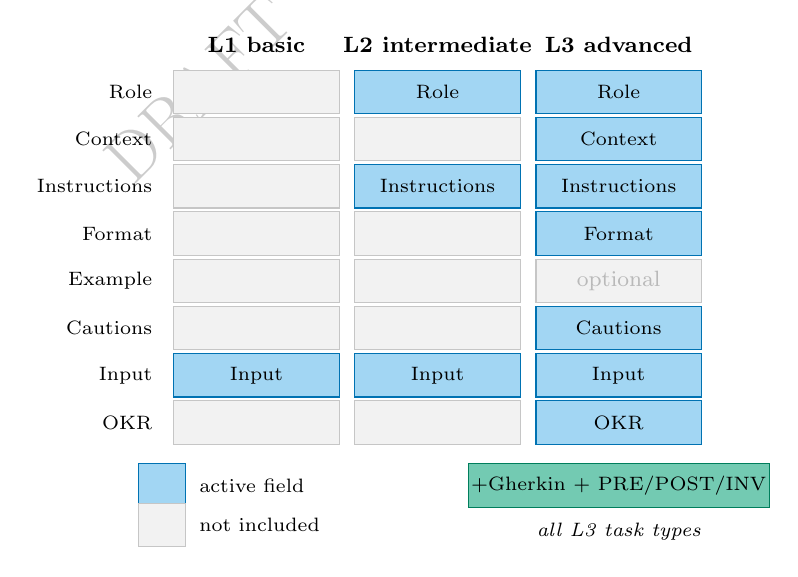
\begin{tikzpicture}[
  cell/.style     = {rectangle, draw, minimum width=2.1cm, minimum height=0.55cm, font=\scriptsize, inner sep=1pt},
  act/.style      = {cell, fill=CUDSkyBlue!55, draw=CUDBlue},
  actO/.style     = {cell, fill=CUDOrange!55, draw=CUDVermilion},
  actG/.style     = {cell, fill=CUDBluishGreen!55, draw=CUDBluishGreen!80!black},
  off/.style      = {cell, fill=gray!10, draw=gray!45, text=gray!55},
  hdr/.style      = {font=\footnotesize\bfseries},
  rowlbl/.style   = {font=\scriptsize, anchor=east}
]
% Column headers
\node[hdr] at (0, 0)  {L1 basic};
\node[hdr] at (2.3, 0){L2 intermediate};
\node[hdr] at (4.6, 0){L3 advanced};

% Row labels
\foreach \y/\lbl in {-1/Role, -2/Context, -3/Instructions, -4/Format,
                     -5/Example, -6/Cautions,-7/Input, -8/OKR}
  \node[rowlbl] at (-1.2, \y*0.6) {\lbl};

% L1 column (only Input active)
\node[off] at (0, -0.6)  {};
\node[off] at (0, -1.2)  {};
\node[off] at (0, -1.8)  {};
\node[off] at (0, -2.4)  {};
\node[off] at (0, -3.0)  {};
\node[off] at (0, -3.6)  {};
\node[act] at (0, -4.2)  {Input};
\node[off] at (0, -4.8)  {};

% L2 column (Role + Instructions + Input)
\node[act] at (2.3, -0.6){Role};
\node[off] at (2.3, -1.2){};
\node[act] at (2.3, -1.8){Instructions};
\node[off] at (2.3, -2.4){};
\node[off] at (2.3, -3.0){};
\node[off] at (2.3, -3.6){};
\node[act] at (2.3, -4.2){Input};
\node[off] at (2.3, -4.8){};

% L3 column (all 6 mandatory + Notices + OKR; Example optional)
\node[act] at (4.6, -0.6){Role};
\node[act] at (4.6, -1.2){Context};
\node[act] at (4.6, -1.8){Instructions};
\node[act] at (4.6, -2.4){Format};
\node[off] at (4.6, -3.0){\footnotesize optional};
\node[act] at (4.6, -3.6){Cautions};
\node[act] at (4.6, -4.2){Input};
\node[act] at (4.6, -4.8){OKR};

% Gherkin + formal-spec annotation under L3 (all three task types)
\node[actG, minimum width=2.4cm, minimum height=0.55cm] at (4.6, -5.6) {+Gherkin + PRE/POST/INV};
\node[font=\scriptsize, anchor=north, align=center] at (4.6, -5.95)
  {\itshape all L3 task types};

% Legend
\node[act, minimum width=0.6cm] at (-1.2, -5.6) {};
\node[anchor=west, font=\scriptsize] at (-0.85, -5.6) {active field};
\node[off, minimum width=0.6cm] at (-1.2, -6.1) {};
\node[anchor=west, font=\scriptsize] at (-0.85, -6.1) {not included};
\end{tikzpicture}
\caption{CLEAR level $\to$ RCIFENI-O gating. Each column shows which of the eight RCIFENI-O fields are activated at a given prompt-quality level. L1 carries only the raw \emph{Input}; L2 adds \emph{Role} + \emph{Instructions}; L3 activates the full mandatory set plus \emph{Notices} and \emph{OKR} (Example remains optional). The L3 problem-solving prompt additionally embeds a Gherkin Given/When/Then acceptance contract. This deterministic gating converts CLEAR's criterion count into a reproducible structural specification.}
\label{fig:rcifeni-o}
\end{figure}

\textbf{Dependent Variable (DV):} AI response quality, measured using the proposed AIOQ-R rubric across five dimensions on a 5-point Likert scale (composite score range: 5--25). Table~\ref{tab:aioq-r} presents the rubric with anchor examples.

\begin{table}[h]
\caption{AIOQ-R Rubric---Five-dimensional AI response quality assessment.}\label{tab:aioq-r}
\centering
\begin{tabular}{@{}lp{3cm}cp{5cm}@{}}
\toprule
\textbf{Dimension} & \textbf{Assessment Focus} & \textbf{Scale} & \textbf{Anchor Examples (L1 / L3 / L5)} \\
\midrule
Accuracy & Technical correctness of information, code, and algorithmic analysis & 1--5 & L1: Critical technical errors causing misconceptions. L3: Correct main ideas with 1--2 minor errors. L5: Fully accurate, independently verifiable. \\
\addlinespace
Completeness & Coverage of all task requirements & 1--5 & L1: Missing $>$50\% of core content. L3: Covers 60--80\% of requirements. L5: 100\% coverage with relevant supplementary information. \\
\addlinespace
Relevance & Alignment between response content and actual learning needs & 1--5 & L1: Off-topic or mismatched context. L3: Topically relevant but wrong difficulty level. L5: Precisely targeted to specified context and level. \\
\addlinespace
Clarity & Logical organization, readability, appropriate examples, and code formatting & 1--5 & L1: Disorganized, no structure, uncommented code. L3: Basic structure but weak transitions. L5: Excellent structure with headings, code blocks, and step-by-step examples. \\
\addlinespace
Learning Value & Stimulation of higher-order thinking~\cite{Anderson2001}; explanations of \emph{why}, comparisons, and reflective questions & 1--5 & L1: Provides answers without explanation. L3: Basic explanations without connecting to broader concepts. L5: Deep explanations, alternative comparisons, open-ended questions promoting analysis. \\
\bottomrule
\end{tabular}
\end{table}

\textbf{Moderator:} AI platform---GPT-4o-mini (OpenAI) vs. GLM-5.1 (Zhipu AI). Both are the same snapshots used in the pilot reported in Section~\ref{sec:pilot} and will remain pinned throughout Phase~2 to prevent silent model updates from confounding results. If either snapshot is deprecated before data collection completes, the study will migrate to the closest successor snapshot and report the migration window together with a re-calibration check. Sampling temperature is held at the provider default for both platforms and the stochastic budget is held identical across conditions; temperature effects on output variance are therefore held constant, not eliminated.

\textbf{Covariate:} Self-reported AI literacy score, measured via a pre-survey instrument adapted from Knoth et al.~\cite{Knoth2024}, used in ANCOVA robustness checks.

\subsection{Experimental Procedure}

The data collection follows three phases over a 14-week semester:

\textbf{Phase 1---Baseline Survey (Weeks 1--2):} A pre-survey (15--20 items) collects demographic data, AI usage frequency, and self-assessed AI literacy. Participants then complete one free-form learning task with their preferred AI tool, with all prompts and responses recorded to characterize natural prompting behaviors.

\textbf{Phase 2---Controlled Experiment (Weeks 6--9):} Each participant completes 18 experimental sessions---3 prompt levels $\times$ 2 platforms $\times$ 3 task types (algorithm explanation, complexity analysis, and problem-solving). Task-order is counterbalanced by a $3 \times 3$ Latin Square: participants are allocated to one of three groups, and each group is assigned a distinct row of the square, guaranteeing that each task type appears equally often in the first, second, and third position across the sample. Prompt-level $\times$ platform order within each sitting is randomised independently per participant using a fixed seed recorded in \texttt{parameters.json}. Prompts are pre-designed and administered directly. Each session starts a fresh conversation. The 18 sessions are distributed across three sittings (6 sessions each), separated by at least 48 hours. Two independent raters score all responses using the AIOQ-R rubric under blind conditions (raters are unaware of the prompt level).

\textbf{Phase 3---Qualitative Interviews (Weeks 9--10):} Semi-structured interviews with 8--10 participants selected via maximum variation sampling. Interview questions explore perceptions of prompt--output relationships, perceived learning value, and awareness of over-reliance risks. All interviews are audio-recorded and fully transcribed.

\textbf{Ethical considerations:} Informed consent is obtained from all participants. All data is anonymized. The study protocol will be submitted for institutional ethics review.

\begin{figure}[!t]
\centering
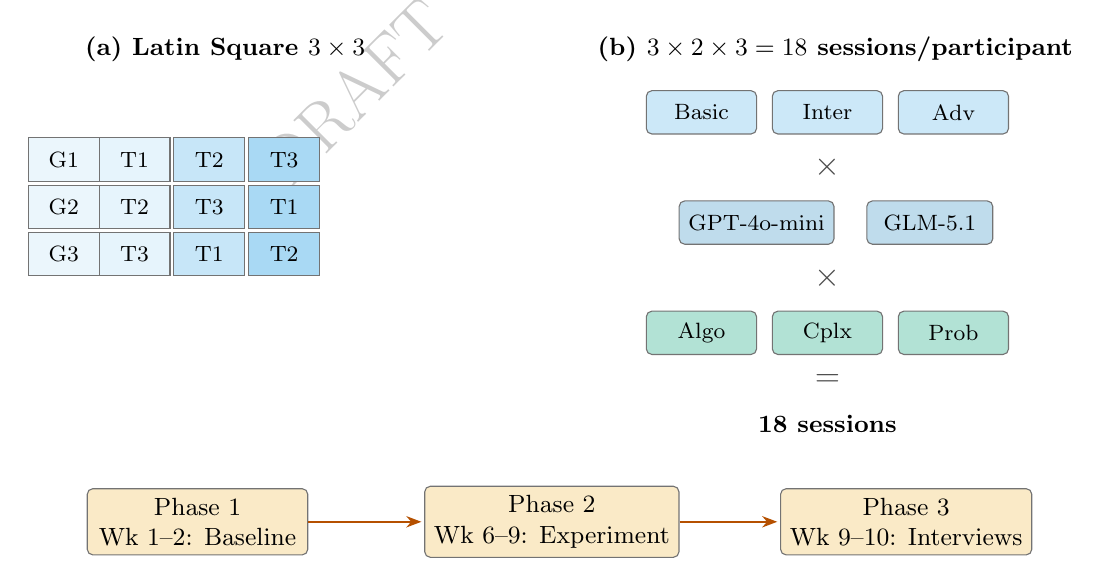
\begin{tikzpicture}[
  every node/.style={font=\footnotesize},
  cell/.style={rectangle, draw=black!55, minimum width=0.9cm, minimum height=0.55cm, align=center, line width=0.4pt},
  sbox/.style={cell, fill=CUDSkyBlue!12},
  proc/.style={rectangle, rounded corners=2pt, draw=black!55, minimum width=1.4cm, minimum height=0.55cm, align=center, line width=0.4pt, font=\footnotesize},
  gprompt/.style={proc, fill=CUDSkyBlue!30},
  gplatform/.style={proc, fill=CUDBlue!25, minimum width=1.6cm},
  gtask/.style={proc, fill=CUDBluishGreen!30},
  phasebox/.style={rectangle, rounded corners=2pt, draw=black!55, minimum width=2.8cm, minimum height=0.8cm, align=center, line width=0.4pt, font=\small, fill=CUDOrange!22},
  arr/.style={->, thick, >=Stealth, draw=CUDVermilion!85!black, shorten >=1pt, line width=0.55pt},
  opsym/.style={font=\large\bfseries, text=black!70}
]

%% (a) Latin Square 3x3 -- CUDSkyBlue gradient left-to-right.
\node[font=\small\bfseries] at (-4.15, 3.4) {(a) Latin Square $3\times3$};
\foreach \i/\row in {1/{T1,T2,T3}, 2/{T2,T3,T1}, 3/{T3,T1,T2}} {
  \node[sbox] at (-6.2, {2.6-\i*0.6}) {G\i};
  \foreach \j/\v [count=\jj from 0] in \row {
    \node[cell, fill=CUDSkyBlue!\the\numexpr15+\jj*18\relax] at ({-5.3+\jj*0.95}, {2.6-\i*0.6}) {\v};
  }
}

%% (b) Multiplicative design 3 x 2 x 3 = 18 with explicit operator symbols.
\node[font=\small\bfseries] at (3.6, 3.4) {(b) $3\times2\times3 = 18$ sessions/participant};
\foreach \x/\lbl in {0/Basic, 1.6/Inter, 3.2/Adv} {
  \node[gprompt] at (\x+1.9, 2.6) {\lbl};
}
\node[opsym] at (3.5, 1.9) {$\times$};
\foreach \x/\lbl in {0/{GPT-4o-mini}, 2.2/GLM-5.1} {
  \node[gplatform] at (\x+2.6, 1.2) {\lbl};
}
\node[opsym] at (3.5, 0.5) {$\times$};
\foreach \x/\lbl in {0/Algo, 1.6/Cplx, 3.2/Prob} {
  \node[gtask] at (\x+1.9, -0.2) {\lbl};
}
\node[opsym] at (3.5, -0.8) {$=$};
\node[font=\small\bfseries] at (3.5, -1.35) {$\mathbf{18}$ sessions};

%% Bottom timeline -- CUDOrange phases, CUDVermilion arrows.
\node[phasebox] (ph1) at (-4.5, -2.6) {Phase~1\\Wk~1--2: Baseline};
\node[phasebox] (ph2) at (0.0, -2.6) {Phase~2\\Wk~6--9: Experiment};
\node[phasebox] (ph3) at (4.5, -2.6) {Phase~3\\Wk~9--10: Interviews};
\draw[arr] (ph1.east) -- (ph2.west);
\draw[arr] (ph2.east) -- (ph3.west);
\end{tikzpicture}
\caption{Experimental design. (a) Latin Square counterbalancing assigns distinct task sequences across 3 participant groups (T1--T3 denote the three task types: algorithm explanation, complexity analysis, problem solving). (b) 3 prompt levels $\times$ 2 platforms $\times$ 3 task types = 18 sessions per participant, distributed across three sittings separated by $\geq$48~hours. Bottom: 14-week mixed-methods timeline.}
\label{fig:design}
\end{figure}

\subsection{Data Analysis Plan}

The analysis strategy comprises four tiers:

\textbf{Primary Analysis:} Two-Way Repeated-Measures ANOVA (Prompt Level $\times$ Platform) is conducted separately for each AIOQ-R dimension and the composite score. Bonferroni-corrected significance level $\alpha' = 0.01$ (i.e., $0.05 / 5$) is applied. Post-hoc pairwise comparisons use Bonferroni correction. Effect sizes are reported as partial $\eta^2$ with 95\% confidence intervals. If sphericity is violated (Mauchly's $p < 0.05$), Greenhouse--Geisser correction is applied. Non-parametric Friedman tests are conducted in parallel as robustness checks.

\textbf{ANCOVA Robustness Check:} ANCOVA with AI literacy as a continuous covariate is performed in parallel to control for confounding effects and verify that the main results (H1) remain significant after accounting for baseline AI literacy variance.

\textbf{LMM Robustness Check:} A Linear Mixed-Effects Model is fitted to handle the nested data structure and potential missing data (MAR). Ceiling effects are assessed via histograms; if maximum scores (5/5) at Level~3 exceed 40\%, supplementary non-parametric analyses are applied.

\textbf{Mixed Methods Integration:} A Joint Display table links (a) AIOQ-R scores by prompt level with natural prompting patterns from Phase~1 to explain outlier patterns, and (b) interaction effects from H3 with interview themes from Phase~3 to explain \emph{why} specific platforms respond differently to advanced prompts on particular task types. Qualitative analysis follows Braun and Clarke's~\cite{Braun2006} six-phase thematic analysis protocol, with inter-rater reliability target of $\kappa \geq 0.67$. Software: SPSS~29 or R (rstatix, emmeans, lme4); NVivo for qualitative coding.

\section{Results}\label{sec:results}

\subsection{Computational Feasibility Pilot}\label{sec:pilot}

A computational pilot verified the end-to-end pipeline before the IRB-gated Phase~2. We sampled $N=\PilotN$ problems with a fixed seed from HumanEval~\cite{Chen2021HumanEval} (164 Python function-completion tasks) and produced \PilotSessions{} sessions across \emph{two} generators --- GPT-4o-mini and GLM-5.1 --- crossed with three CLEAR-grounded prompt levels and three pedagogical framings (algorithm explanation, complexity analysis, problem solving). GLM-5.1 contributed 76 of the 90 planned sessions; 14 calls were dropped because the model's inference on the most structurally heavy prompts exceeded the per-call 180-second wall-time budget (attrition rate $\approx 16\%$, concentrated on complexity-analysis L2/L3 cells). Prompt levels were instantiated through the RCIFENI-O framework (see Appendix), so \emph{level} is a structural-completeness variable rather than a free-form verbal directive. An automatic GPT-4o-mini judge scored each response on the five AIOQ-R dimensions on a 1--5 Likert scale, producing a composite in the 5--25 range. A Friedman test across the three prompt levels, treating each (problem, task-type, platform) triple as a repeated block, yielded $\chi^2(\PilotFriedmanDF)=\PilotFriedmanChi$, $p=\PilotFriedmanP$, Kendall's $W=\PilotKendallW$.

\begin{figure}[!t]
\centering
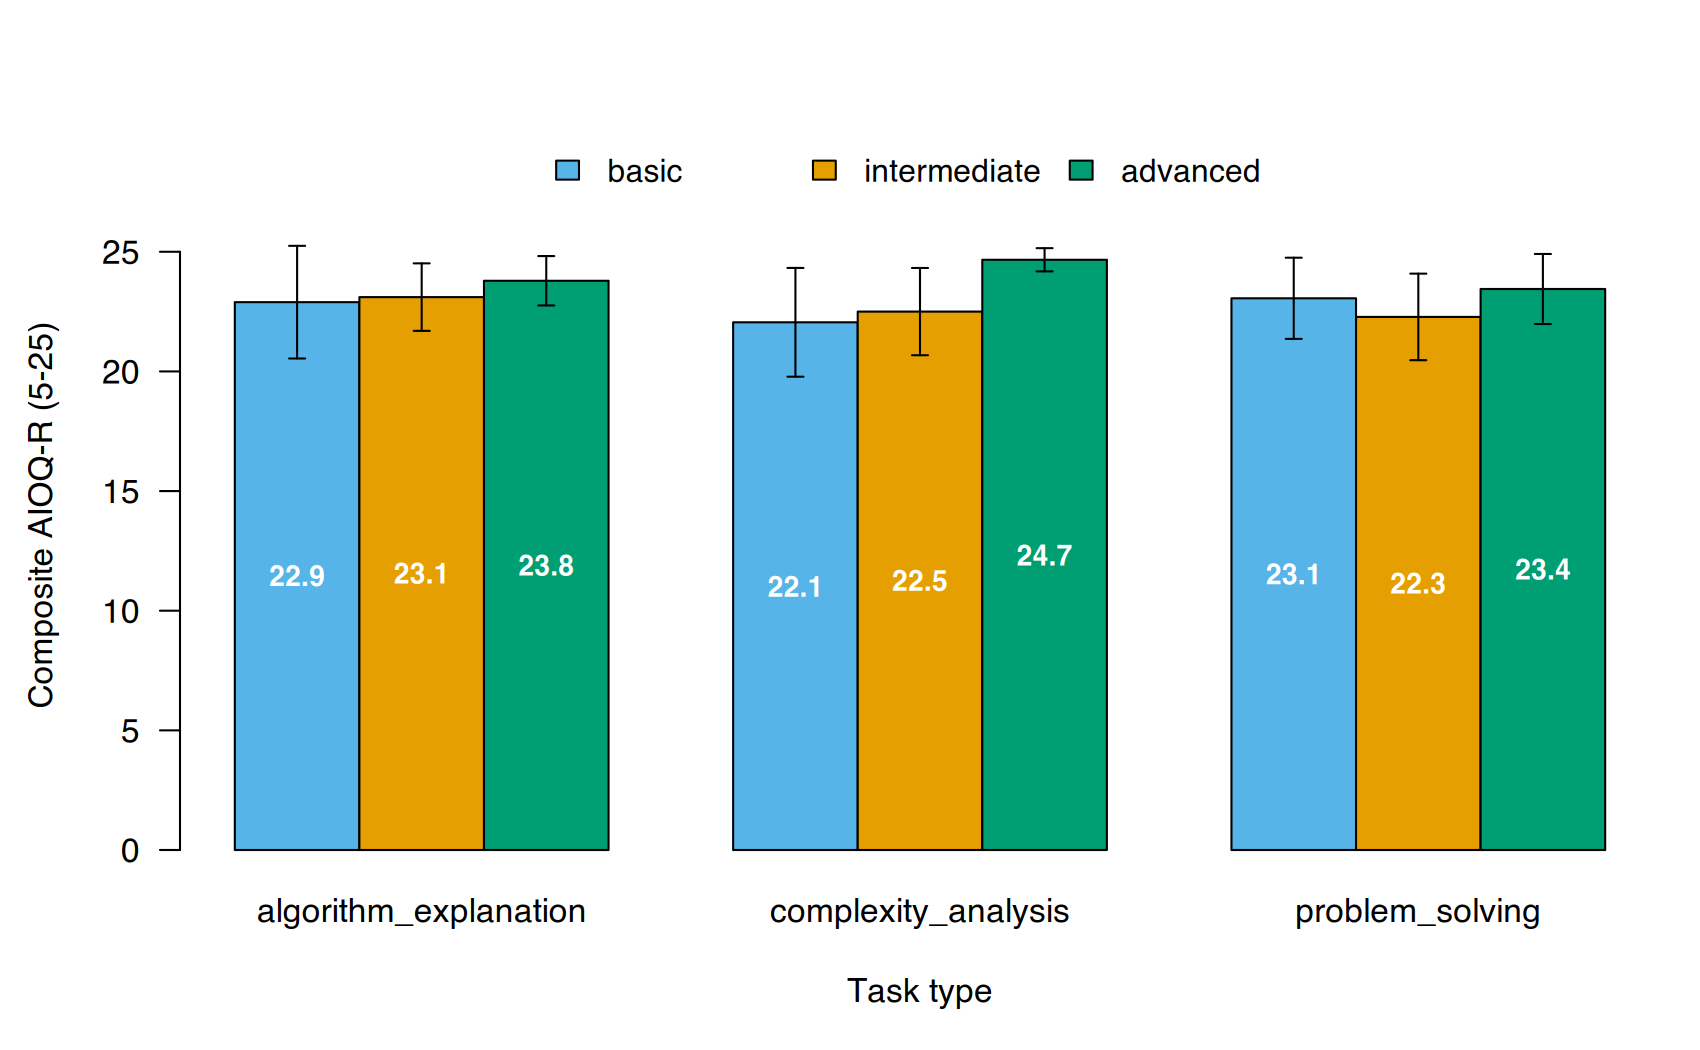
\includegraphics[width=0.85\linewidth]{figures/pilot_bars}
\caption{Pilot composite AIOQ-R (mean$\pm$SD across \PilotN{} HumanEval problems per cell), rated by a GPT-4o-mini judge, by CLEAR prompt level (basic, intermediate, advanced) and task framing. CUD colour-universal palette.}
\label{fig:pilot-bars}
\end{figure}

\begin{figure}[!t]
\centering
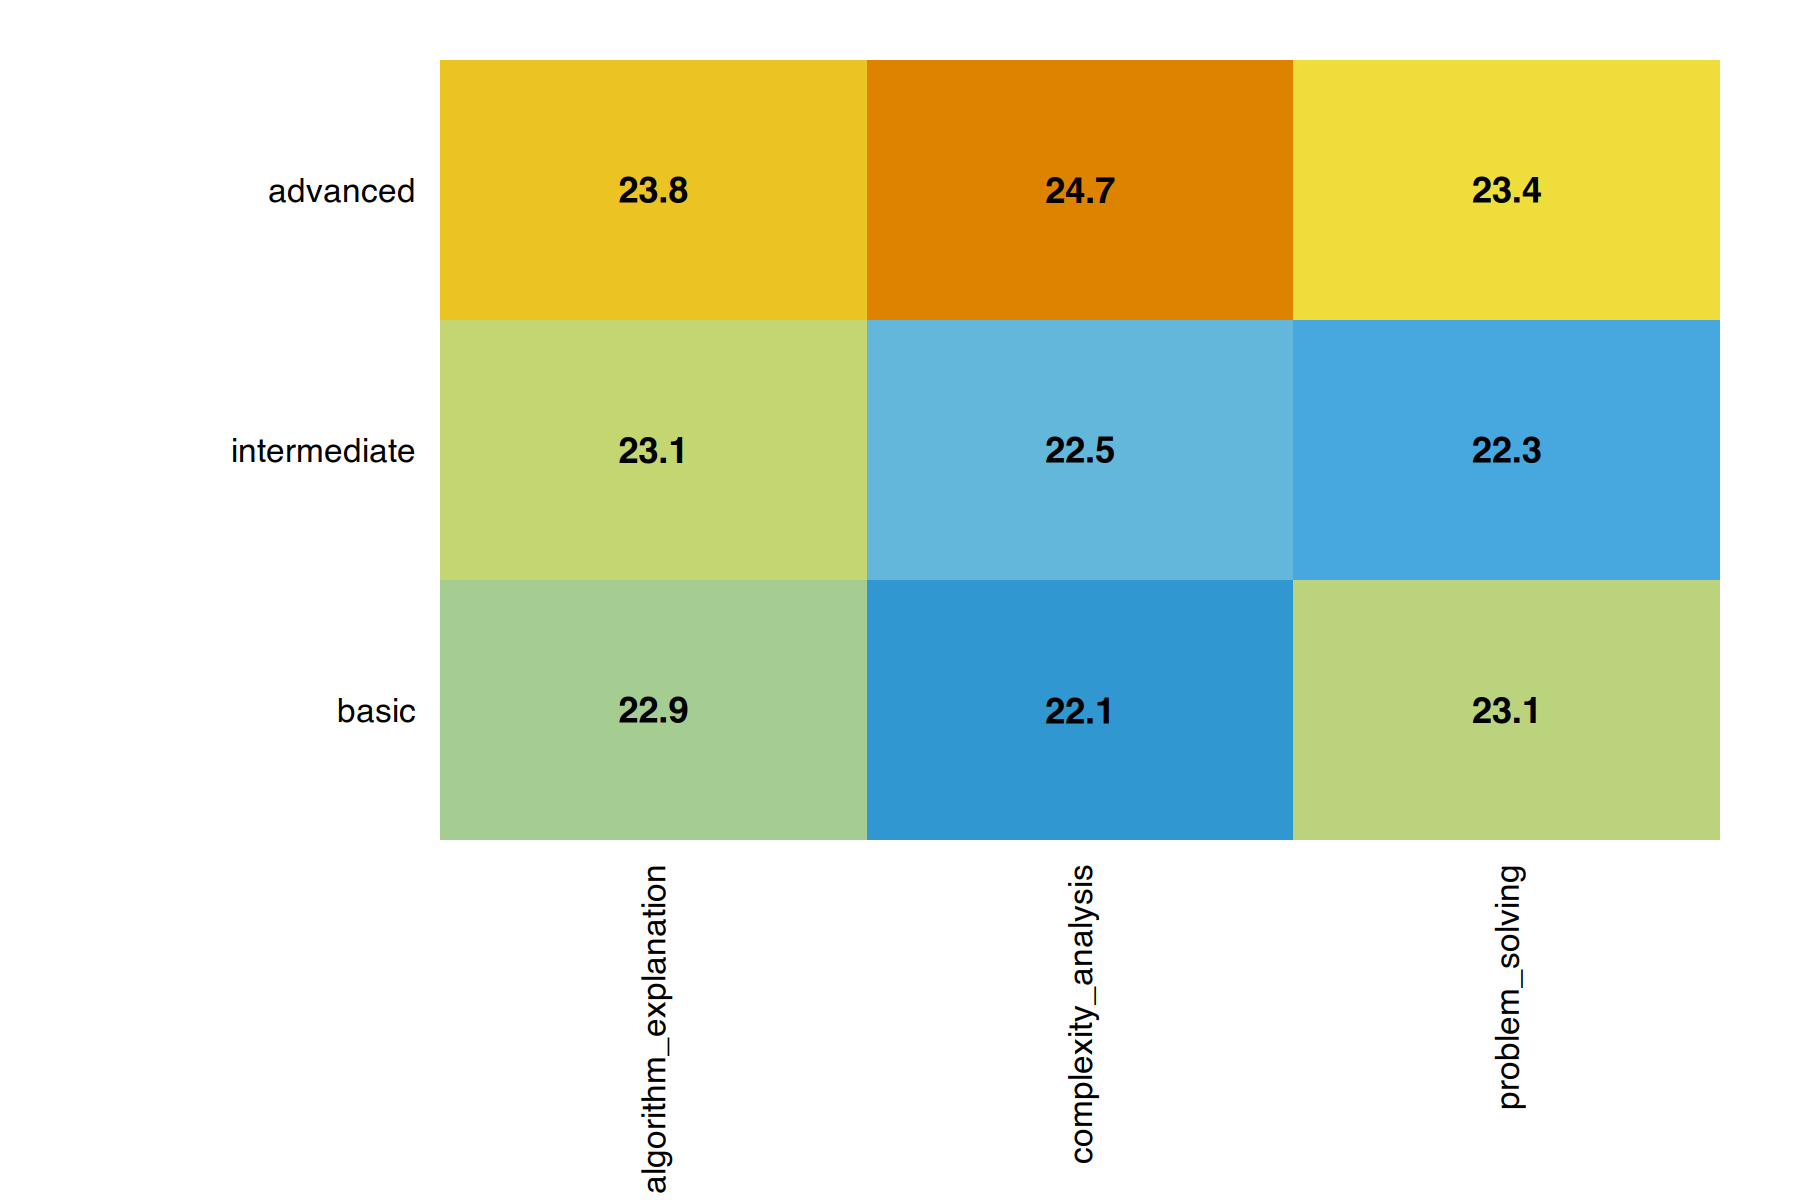
\includegraphics[width=0.72\linewidth]{figures/pilot_heatmap}
\caption{Cell-mean heatmap of pilot composite AIOQ-R across the same nine conditions as Fig.~\ref{fig:pilot-bars}. The narrow observed range reflects LLM-as-judge ceiling inflation; a calibrated human panel in Phase~2 is expected to expand it.}
\label{fig:pilot-heatmap}
\end{figure}

Per-cell composite means (basic / intermediate / advanced) were \PilotAlgoBasic{} / \PilotAlgoInt{} / \PilotAlgoAdv{} for algorithm explanation, \PilotCxBasic{} / \PilotCxInt{} / \PilotCxAdv{} for complexity analysis, and \PilotPsBasic{} / \PilotPsInt{} / \PilotPsAdv{} for problem solving. Contrary to the literature-anchored monotonic expectation $L3>L2>L1$, the pilot shows no such ordering on these compact HumanEval tasks: automatic scores cluster near the top of the scale and the RCIFENI-O-grounded L3 prompts, even with embedded Gherkin and PRE/INV/POST/ERR specifications, do not outperform the bare L1 input. Three caveats apply. \emph{First}, LLM-as-judge raters are known to inflate scores and compress between-level variance relative to calibrated human raters~\cite{Liu2023}, so Kendall's $W$ here is a \emph{floor} estimate of the effect size a human panel is expected to detect, not a substitute for the pre-registered partial $\eta^2\geq0.06$ target. \emph{Second}, HumanEval tasks are compact single-function problems whose solutions fit in a single short response regardless of prompt structure, which limits the room for prompt engineering to help; richer open-ended learning tasks in Phase~2 are expected to widen level differences. \emph{Third}, the highly structured L3 instructions (role + context + Cautions + OKR + Gherkin + formal spec) appear to over-specify compact tasks: on small HumanEval problems the structural overhead seems to distract rather than guide, an effect the longer, open-ended Phase~2 tasks are not expected to reproduce. \emph{Fourth}, the 14 dropped GLM-5.1 calls were not uniformly distributed: they concentrated on complexity-analysis L2/L3 cells, the same cells in which GLM-5.1 shows its largest gains. Readers should therefore treat the GLM complexity-analysis effect as an \emph{upper-bound estimate} until Phase~2 collects complete paired data; the direction of any bias is towards overestimation, not confirmation.

\subsection{Phase~2 Hypotheses}\label{sec:phase2-hypo}

Pilot signals inform, but do not supersede, the pre-registered hypotheses for the human-participant Phase~2.

\textbf{H1---Prompt Quality Main Effect.} We expect a statistically significant monotonic increase in composite AIOQ-R scores across the three prompt levels: Level~3 (advanced) $>$ Level~2 (intermediate) $>$ Level~1 (basic). The anticipated effect size is partial $\eta^2 \geq 0.06$ (medium effect), grounded in the effect sizes reported by Sawalha et al.~\cite{Sawalha2024} ($d = 0.69$--$0.94$) and the 33\% performance gain documented by Kumar et al.~\cite{Kumar2025}. Among the five AIOQ-R dimensions, the largest gains from Level~1 to Level~3 are expected on \emph{Completeness} and \emph{Learning Value}, as advanced prompts with explicit context and CoT instructions should activate more comprehensive and pedagogically rich responses through the Reasoning Scaffolding mechanism~\cite{Wei2022}. \emph{Accuracy} improvements are anticipated to plateau between Level~2 and Level~3, since both intermediate and advanced prompts sufficiently reduce ambiguity to elicit factually correct responses.

\textbf{H2---Platform Main Effect.} We hypothesize a statistically significant difference in composite AIOQ-R scores between GPT-4o-mini and GLM-5.1, though the direction is exploratory. Pilot evidence (Section~\ref{sec:pilot}) suggests GLM-5.1 may show larger gains when prompt structural completeness increases, while GPT-4o-mini hits a ceiling earlier. The hypothesis therefore captures both a main-effect and a ceiling-sensitivity prediction.

\textbf{H3---Interaction Effect.} We anticipate a significant Prompt Level $\times$ Platform interaction, manifesting as differential sensitivity to prompt structural completeness across task types. Specifically, GLM-5.1 is expected to show larger L1$\to$L3 gains on tasks that reward explicit derivation (complexity analysis), while GPT-4o-mini is expected to show a flatter profile because its L1 responses already saturate the judge's scale on compact HumanEval-style problems. This pattern, already visible in the pilot, would indicate that the mechanisms through which prompt quality influences output are architecture-dependent.

\textbf{Qualitative Expectations.} The semi-structured interviews are expected to reveal: (a) a general awareness among students that better prompts yield better responses, but limited knowledge of specific techniques; (b) a tension between perceived usefulness of AI and concerns about over-reliance; and (c) platform-specific preferences that may explain interaction patterns observed in the quantitative data. The Joint Display integration is expected to identify convergent patterns where high-scoring participants in Phase~2 also exhibited multi-turn critical engagement strategies in Phase~1.

\section{Discussion}\label{sec:discussion}

\subsection{Theoretical Implications}

The anticipated results carry several theoretical implications. First, confirmation of H1 would extend the Knoth et al.~\cite{Knoth2024} causal chain model (AI Literacy $\rightarrow$ Prompt Quality $\rightarrow$ Output Quality) by providing \emph{controlled experimental} evidence---advancing beyond the correlational survey design of the original study. By standardizing prompts across participants, this design isolates the effect of prompt quality on output independently of individual AI literacy, representing a methodological contribution.

Second, the three cognitive mechanisms proposed in this study---Ambiguity Reduction, Task Representation Alignment, and Reasoning Scaffolding---provide a theoretically grounded explanation for \emph{how} prompt quality influences each AIOQ-R dimension, bridging Cognitive Load Theory~\cite{Sweller1988} with LLM processing dynamics. The TAM2 framework~\cite{Venkatesh2000} further provides a behavioral lens for interpreting student perceptions of AI output quality and usefulness. If the anticipated differential patterns across dimensions are confirmed (e.g., larger effects on Learning Value than Accuracy at advanced levels), this would support the hypothesis that these mechanisms operate through distinct pathways rather than a unitary quality construct.

Third, confirmation of H3 would challenge the implicit assumption in the literature that prompt--response dynamics are platform-invariant, providing evidence that the CLEAR framework's effectiveness may be modulated by model architecture. This has implications for both the generalizability of existing prompt engineering research and the design of platform-specific pedagogical guidelines.

\subsection{Practical Implications}

The study's practical contributions center on three deliverables. First, the validated AIOQ-R rubric (target: CVI $\geq 0.80$, $\kappa \geq 0.70$) provides a reusable assessment instrument for researchers and educators evaluating AI-generated content in technical education contexts. Unlike existing unidimensional scales, AIOQ-R's inclusion of Learning Value ensures that pedagogical effectiveness---not merely technical accuracy---is assessed.

Second, the 12 standardized prompts (4 tasks $\times$ 3 levels) serve as both experimental stimuli and practical training materials. These can be adapted into prompt engineering workshops for IT curricula, directly addressing the gap identified by Lee and Palmer~\cite{Lee2025} regarding the absence of formal prompt instruction in university programs.

Third, if platform-specific strengths are confirmed (H2, H3), the results inform evidence-based tool selection guidelines: students could be advised to use specific platforms for specific task types, optimizing their AI-assisted learning outcomes.

\subsection{Limitations and Future Work}

Several limitations should be noted. First, this paper presents a research design and expected results; actual empirical data has not yet been collected. The hypotheses and anticipated patterns are grounded in prior evidence but remain to be confirmed through experimentation. Second, the use of pre-designed controlled prompts reduces ecological validity compared to naturalistic usage; this is partially mitigated by the Phase~1 baseline observation and Phase~3 interviews. Third, the study is conducted at a single institution in Vietnam with a relatively small sample ($N = 30$--$40$), limiting generalizability. Fourth, the AIOQ-R rubric's Learning Value dimension involves inherently subjective judgment, even with anchor examples and blind rating protocols. Fifth, the novelty claim regarding the Southeast Asian context is scoped to English-language peer-reviewed literature indexed at the time of writing; non-English preprints from Vietnamese, Thai, Indonesian, or other regional sources may describe analogous designs that were not captured by our search protocol.

Future work should include: (a) execution of the proposed experiment and analysis of actual data; (b) longitudinal studies examining whether prompt training effects persist over time; (c) extension to additional platforms (e.g., Gemini, open-source models); (d) replication in non-IT disciplines to test domain transferability; and (e) automated evaluation approaches (e.g., LLM-as-judge) to complement human rater assessment and enable larger-scale studies.

\section{Conclusion}\label{sec:conclusion}

This paper presents the design of a controlled within-subjects experiment to investigate the impact of prompt quality on generative AI response efficacy across two competing platforms---GPT-4o-mini and GLM-5.1---in the context of IT students performing academic learning tasks. The study makes three primary contributions.

First, to the authors' knowledge, it proposes one of the earliest cross-platform controlled experimental designs for studying prompt--response dynamics in a Southeast Asian educational context, addressing the geographic and methodological gaps in the existing literature. The within-subjects design with Latin Square counterbalancing and fixed API parameters ensures rigorous control over confounding variables.

Second, it introduces the AIOQ-R rubric, a five-dimensional assessment instrument that uniquely incorporates Learning Value---anchored to Bloom's taxonomy---alongside technical accuracy, completeness, relevance, and clarity. The planned validation protocol (CVI $\geq 0.80$, inter-rater $\kappa \geq 0.70$) is designed to produce a reusable tool for the research community.

Third, it proposes an integrated theoretical framework combining the CLEAR framework for prompt operationalization, Cognitive Load Theory for mechanistic explanation, and TAM2 for behavioral interpretation, providing a comprehensive lens through which prompt--response interactions can be understood.

We anticipate that the empirical results will confirm that prompt quality significantly improves AI response quality, with platform-specific interaction effects across task types. These findings, once validated, will provide evidence-based foundations for integrating prompt engineering into IT curricula and developing practical prompt-writing guidelines for students navigating an AI-augmented educational landscape.

\section*{Declarations}\label{sec:declarations}

\noindent\textbf{Funding:} No external funding; API and computational costs borne by the authors' institutions.
\textbf{Conflicts of Interest:} None declared; the authors have no commercial or advisory relationship with OpenAI or Anthropic.
\textbf{Ethics Approval:} Protocol will be submitted to the IRB of FPT University (HCMC) prior to Phase~1; no human-subjects data is collected before approval, and the reference will be reported in the revised submission. All participants provide written informed consent; data is de-identified at capture.
\textbf{Data and Code Availability:} Code skeleton (Python and R with synthetic-data exemplars) is released at the project repository (anonymised for review). The pre-registration record will be deposited on OSF and the DOI added to the camera-ready version. Phase~2 empirical data will be released under CC~BY~4.0 on acceptance of the follow-up paper.
\textbf{Author Contributions (CRediT):} Nguyen--Conceptualization, Methodology, Writing~(Original Draft), Project Administration; Ho-Van--Methodology, Statistical Design, Writing~(Review~\& Editing), Supervision; Lam--Software, Validation, Data Curation, Writing~(Review~\& Editing).
\textbf{Generative AI Usage:} GPT-4o-mini and GLM-5.1 are the \emph{object of study} and are used solely as controlled experimental platforms; no generative AI was used to draft or substantively revise the manuscript beyond minor grammar suggestions, per the 2023 COPE/ICMJE/Springer AI-authorship guidance.
\textbf{ORCID:} All three authors' ORCID iDs will be finalised in the camera-ready version.

{\footnotesize
\bibliographystyle{splncs04}
\bibliography{references}
}

% Appendix C — RCIFENI-O CLEAR-level operationalisation summary.
% No external paths in paper body. Full verbatim templates in the
% supplementary material released with the paper.

\section*{Appendix: Prompt Templates (RCIFENI-O)}\label{sec:appendix-a}

All nine prompts (three CLEAR levels $\times$ three pedagogical
framings) and the AIOQ-R judge prompt are assembled with an eight-field
framework we refer to as RCIFENI-O: \textbf{R}ole, \textbf{C}ontext,
\textbf{I}nstructions, \textbf{F}ormat, \textbf{E}xample (optional),
\textbf{N}otices (cautions), \textbf{I}nput, \textbf{O}KR. The CLEAR
level~\cite{Lo2023} therefore maps deterministically to
\emph{structural completeness}, not merely a criterion count.

\begin{table}[htbp]
  \centering
  \caption{CLEAR level $\to$ RCIFENI-O sections instantiated. Every L3
           prompt (all three task framings) additionally embeds a Gherkin
           Given/When/Then acceptance contract and a PRE/INV/POST/ERR
           formal specification.}
  \label{tab:clear-rcifeni}
  \begin{tabular}{lll}
    \toprule
    CLEAR level & RCIFENI-O sections                          & Gherkin + formal spec \\
    \midrule
    L1 basic        & Input only                              & no  \\
    L2 intermediate & Role + Instructions + Input             & no  \\
    L3 advanced     & Role + Context + Instructions + Format  & yes \\
                    & \quad + Cautions + OKR + Input          & (all L3 task types) \\
    \bottomrule
  \end{tabular}
\end{table}

The full verbatim text of all nine templates and the AIOQ-R judge prompt
is distributed in the supplementary material that accompanies the paper.


\end{document}
